
\documentclass[12pt,a4paper]{article}
%\input epsf
\usepackage{wallpaper}
\usepackage{float}
\usepackage[T1]{fontenc}
\usepackage[utf8]{inputenc}
\usepackage{graphicx}
\usepackage{amsmath}
\usepackage[english]{babel}
\usepackage[small]{caption}
\usepackage{amsbsy}
\usepackage{amssymb}
\usepackage{amsthm}
\usepackage{amscd}
\usepackage{amsfonts}
\usepackage{enumerate}
\usepackage{subfig}
\usepackage{ upgreek }
\usepackage{graphicx}
\usepackage{listings}



%\decimalpoint
\pagestyle{empty}
\setlength{\voffset}{0cm}
\setlength{\headheight}{-2.5cm}
\setlength{\oddsidemargin}{0in}
\setlength{\textwidth}{6.5in}
\setlength{\textheight}{9.5in}
\setlength{\captionmargin}{60pt}
\setlength{\parindent}{0pt}
\newcommand{\listaproblemas}[3]{%
\noindent \rule{\textwidth}{0.02in} \\[0.1cm]
\noindent {\bf #1} \hfill {\bf #2} \\[0.2cm]
\centerline{\Large\bf #3}\\
\noindent \rule{\textwidth}{0.02in} \\[0.1cm]}
\newcommand{\raya}{\centerline{\rule{0.5\textwidth}{0.02in}}}

%_______________________________________________________________________________
%                                      Definiciones particulares de este archivo

\usepackage{color}
\usepackage{colordvi}
\usepackage{fancyhdr}

\usepackage{paralist}
\usepackage{url}
\usepackage{bbm}
\usepackage{nopageno}

\pagestyle{fancy}
\fancyhf{}
\fancyfoot[R]{\vspace{1.75cm} \thepage}

\newtheorem{prob}{}
\newtheorem*{teo}{Theorem}
\newtheorem*{defi}{Definition}
\newtheorem*{obs}{Observation}
\newcommand{\vsh}{\vskip .15cm}
\newcommand{\R}{\mathbb R}
\def\headrulewidth{0.0mm}
\def\footrulewidth{0.0mm}%

\definecolor{blau}{rgb}{0,0.459,0.612}

\newcommand{\cA}{\mathcal{A}}
\newcommand{\cS}{\mathcal{S}}
\DeclareMathOperator{\conv}{conv}
\DeclareMathOperator{\New}{New}
\DeclareMathOperator{\area}{area}
\newcommand{\RR}{\mathbbm{R}}
\newcommand{\CC}{\mathbbm{C}}



\newcommand{\bm}[1]{\text{\boldmath $#1$\unboldmath}}  % vectorial function
\newcommand{\vect}[1]{\mathbf{#1}}                     % vectors
\newcommand{\mat}[1]{\mathbf{#1}}                      % matrices

\providecommand{\abs}[1]{\lvert#1\rvert}
\def\A{\mat{A}}
\def\B{\mat{B}}
\def\u{\vect{u}}
\def\f{\vect{f}}
\def\b{\vect{b}}
\def\x{\vect{x}}

%_______________________________________________________________________________
%                                      Caratula
\begin{document}

\begin{center}{\Large{\sc ASSIGNMENT 4, discrete geometry }}\end{center}

\begin{center}{\textit{December, 10th 2018}}\end{center}

\begin{center}{\sc{Marta Bustins, Esteve Tarragó, Marta González}
}\end{center}

\bigskip


\begin{enumerate}
\item Definition 9.2 in Ziegler's \emph{Lectures on Polytopes} constructs the linear map
  \[
    P
    \ \xrightarrow{\pi^c}\ 
    Q^c :=
    \Big\{ \binom{\pi(x)}{cx} : x\in P\Big\}
    \ \subset \
    \RR^{q+1}
  \]
  from a projection $\pi:P\subset\RR^p\to Q\subset\RR^q$ and a linear function $c\in(\RR^q)^\star$.
  Is it possible to give an algorithm to determine the set of lower faces $\mathcal L^\downarrow(Q^c)$ of $Q^c$ from just the set of facet normals of~$Q$, the projection~$\pi$, and the linear function~$c$, without running a convex hull algorithm on $Q^c$?
  
  \bigskip
  It doesn't exist such a deterministic algorithm because for a given input it should always return the same output. In the following examples (rectangle and triangle), the input of the algorithm is the same and the output should be different.
  
    \begin{figure}[H]
    \centering
    \begin{minipage}{0.45\textwidth}
        \centering
			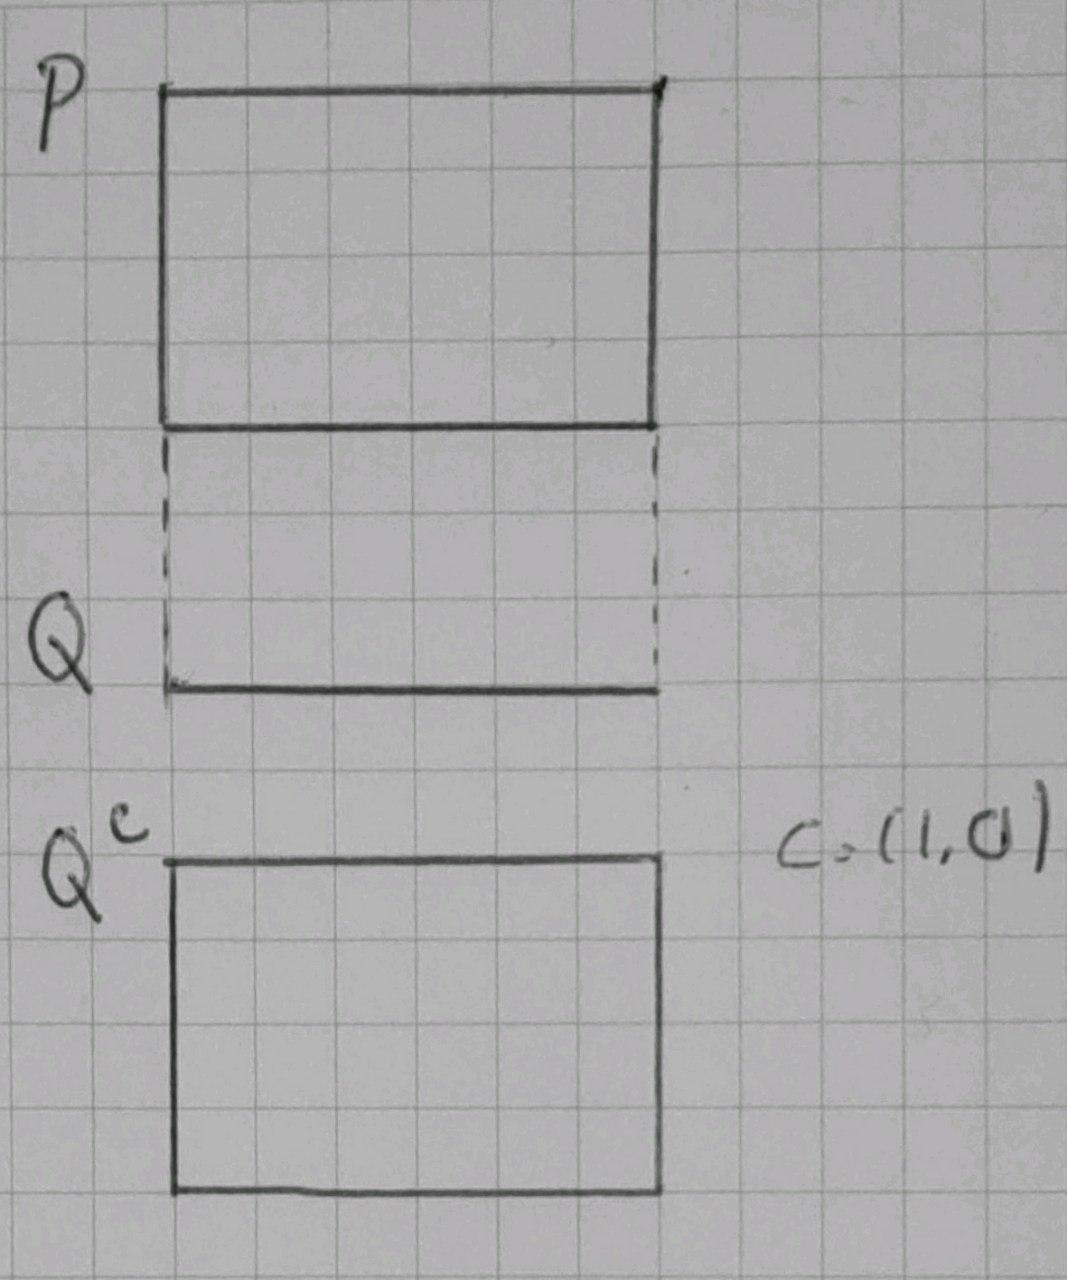
\includegraphics[width=6cm]{A.jpg}
        %\caption{first figure}%
    \end{minipage}\hfill
    \begin{minipage}{0.45\textwidth}
        \centering
			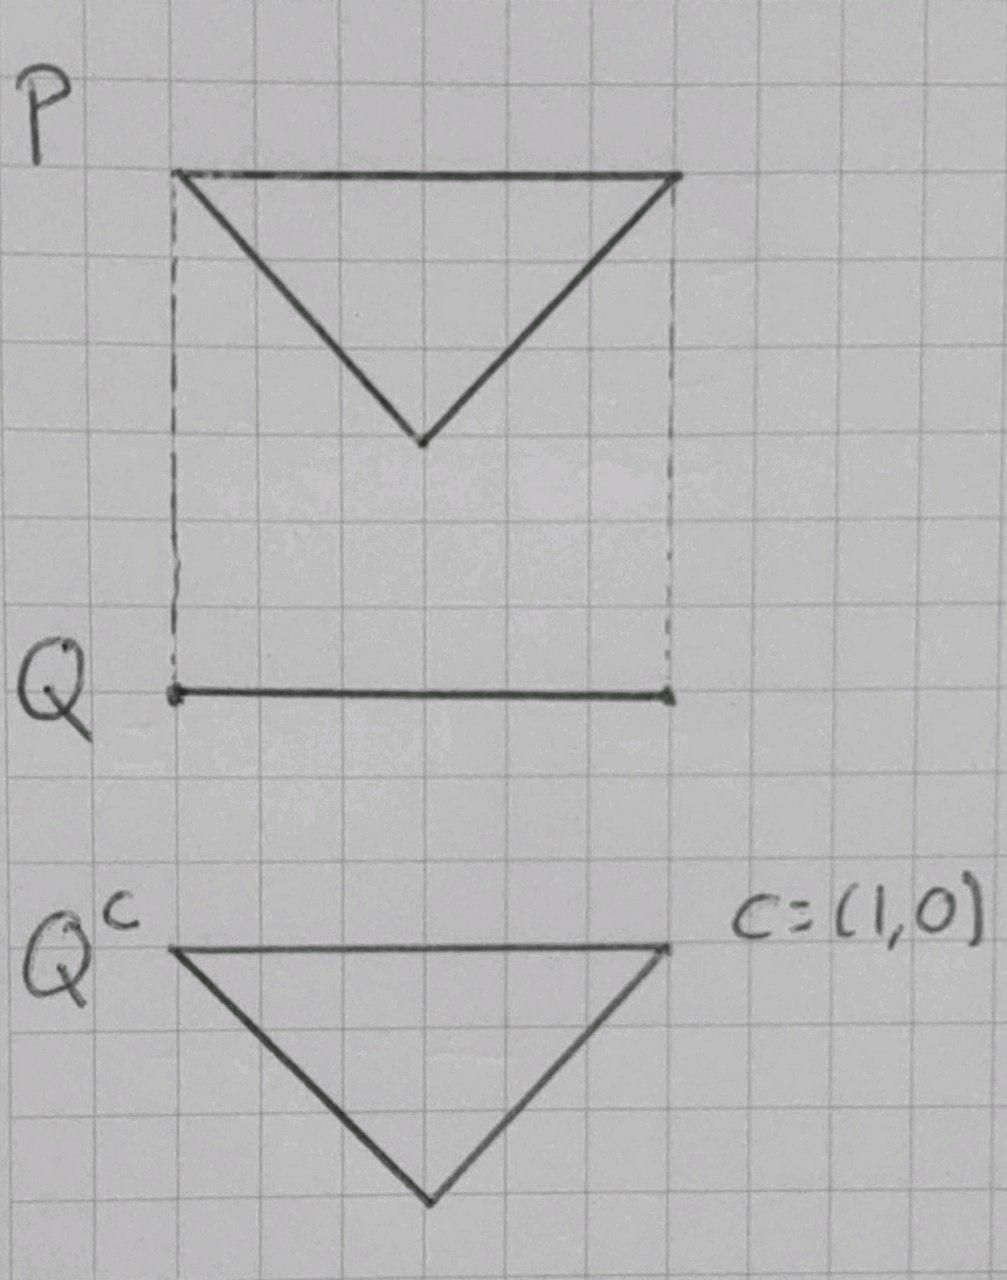
\includegraphics[width=6cm]{B.jpg}
        %\caption{second figure}%
    \end{minipage}
\end{figure}

The input of the algorithm is the set of facet normals of $Q$, the projection $\pi$ (which is removing the second coordinate) and the liniear function c:=(1,0). And the lower faces of $Q^c$ are different in each case.

  \bigskip\bigskip
\item Show that
  \[
    \int_P f(x)\,\text{d}x
    \ = \
    vol(P) \cdot f(p_0)
  \]
  for any polytope $P$ and linear function $f$, where $p_0 = \frac{1}{vol(P)}\int_P x\,\text{d}x$ denotes the barycenter of $P$.
  \bigskip
  
  Let $f$ be a linear function $f:\mathbb{R}^d\longrightarrow\mathbb{R}^n$.
  Then $f$ can be expressed as $f(x)=Ax+b$ where $A$ is a $nxd$ matrix and $b$ is a $nx1$ vector. Then:
  
  \begin{equation*}
       \int_P f(x)\,\text{d}x= \int_P Ax+b\,\text{d}x = A\int_P x\,\text{d}x + b\int_P \,\text{d}x =  (vol P) \bigg(\frac{A}{vol(P)}\int_P x\,\text{d}x + b\bigg) = vol(P)*f(p_0)
  \end{equation*}
  where $p_0 = \frac{1}{vol(P)}\int_P x\,\text{d}x$ is the barycenter of $P$.
  \bigskip
\item Complete the proof of Theorem 9.6 in Ziegler's \emph{Lectures on Polytopes}.
  
\end{enumerate}
\begin{defi}
Let $\gamma$ be a section. $\gamma$ is a tight section if and only if $\mathrm{Im}\gamma=\bigcup_{F\in\mathcal{F}}F$ for some $\mathcal{F}\subseteq\mathcal{L}\left(P\right)$.
\end{defi}
\begin{obs}
If $\gamma$ is a section but it is not tight, then there exists $p\in\mathrm{Im}\gamma$ such that $p\not\in\bigcup_{F\in\mathcal{F}}F$ for any $\mathcal{F}\subseteq\left\lbrace\mathrm{proper\,faces\,of\,P}\right\rbrace$.
\end{obs}

%\textcolor{red}{crec que falta teorema al que es refereix la prova} \textcolor{blue}{A veure, aquí la intenció era posar el teorema TEOREMA, en plan abans de posar-lo primer fixem nocions i fem alguna observació,i després doncs TEOREMA: bla bla bla DEMOSTRACIÓ: bla bla bla perquè crec que quedaria una mica més endraçat... Però si teniu altres opcions endavant!}



\textit{Proof}. Let $\gamma$ and $\rho$ be two sections of $P$, and let $\lambda\in\mathbb{R}$. Then $\lambda\gamma+\left(1-\lambda\right)\rho$ is continuous since it is a linear combination of two continuous functions, and 
\begin{align*}
    \pi\left(\lambda\gamma+\left(1-\lambda\right)\rho\right)\left(x\right)&=\pi\left(\lambda\gamma\left(x\right)+\left(1-\lambda\right)\rho\left(x\right)\right)\\
    &=\lambda\pi\left(\gamma\left(x\right)\right)+\left(1-\lambda\right)\pi\left(\rho\left(x\right)\right)\quad\qquad\mathrm{Since\,}\pi\mathrm{\,is\,linear}\\
    &=\lambda x+\left(1-\lambda\right)x\qquad\qquad\qquad\qquad\quad\;\mathrm{Since\,}\gamma\mathrm{\,and\,}\rho\mathrm{\,are\,sections}\\
    &=x\\
\end{align*}
so any convex combination of sections is a section (seen just by 2 sections, but repeating this argument by induction can be easily proved). In particular, this shows that $\Sigma\left(P,Q\right)$ is convex, since for any $x$, $y\in\Sigma\left(P,Q\right)$, $x=\frac{1}{\mathrm{volQ}}\int_Q\gamma\left(s\right)ds$, $y=\frac{1}{\mathrm{volQ}}\int_Q\rho\left(s\right)ds$, $\gamma$, $\rho$ two sections and $\lambda\in\left[0,1\right]$ we get that
    $$\lambda\frac{1}{\mathrm{volQ}}\int_Q\gamma\left(s\right)ds+\left(1-\lambda\right)\frac{1}{\mathrm{volQ}}\int_Q\rho\left(s\right)ds=\frac{1}{\mathrm{volQ}}\left(\int_Q\left(\lambda\gamma\left(s\right)\left(1-\lambda\right)\rho\left(s\right)\right)ds\right)\in\Sigma\left(P,Q\right)$$
since convex combinations of sections is a section, as we have seen. Moreover, $\Sigma\left(P,Q\right)\subseteq\pi^{-1}\left(r_0\right)$ since, for any $x\in\Sigma\left(P,Q\right)$, $x=\frac{1}{\mathrm{volQ}}\int_Q\gamma\left(s\right)ds$, $$\pi\left(x\right)=\pi\left(\frac{1}{\mathrm{volQ}}\int_Q\gamma\left(y\right)dy\right)=\frac{1}{volQ}\int_Q\pi\left(\gamma\left(y\right)\right)dy=\frac{1}{volQ}\int_Qydy=r_0.$$ On the other hand, $\pi\colon\mathbb{R}^p\to\mathbb{R}^q$ as afine function can be written as $\pi=\pi_l+r_0$, where $\pi_l\colon\mathbb{R}^p\to \mathbb{R}^q$ is a linar function. Hence, in order to find $\mathrm{dim}\pi^{-1}\left(r_0\right)$ it suffices to find $\mathrm{dim}\pi^{-1}_l\left(0\right)=\mathrm{dim\,ker}\pi_l$. By the first isomorphism theorem we have $$\mathrm{dim\,ker}\pi_l=\mathrm{dim\,P}-\mathrm{dim\,Q}.$$ Thus, $\Sigma\left(P,Q\right)$ has dimension $\mathrm{dim\,P}-\mathrm{dim\,Q}$ at most.

Since tight sections correspond to some subsets of $\mathcal{L}\left(P\right)$, there will be a finite number of tight sections.

\textit{Claim.} Every section $\gamma$ not tight can be expressed as a convex combination of 2 other sections.

As we have seen, $\Sigma\left(P,Q\right)$ is convex, whose points are given by the sections $\gamma\colon Q\to P$. Then, since every interior point of a convex set can be expressed as convex combinations of other points of the set, but the vertices, and the only sections that cannot be written as convex combinations of other sections are the tight ones, we have that the vertices of $\Sigma\left(P,Q\right)$ correspond to the tight sections. Then, $\Sigma\left(P,Q\right)$ is the convex hull of a finite number of points, so it must be a polytope.

%\textcolor{red}{Feu-li una ullada! Fins aquí és tot el que tenia al paper jo, ara ja toca veure que, de fet, les tight sections corresponen a les $\pi$-coherent tight subdivisions... Si hi ha algo que no s'entén canvieu-ho :) }
\end{document}